\chapter{Reti neurali}
\section{Neuroni biologico}
L'idea alla base delle reti neurali è quella di replicare, grazie all'utilizzo
di un computer, il funzionamento del cervello umano. Per fare ciò si è utile
farsi un idea su come funziona il cervello. Esso è composto da un insieme di
neuroni molto grande di neuroni che comunicano tra di loro. Ogni neurone è composto
nel seguente modo:
\begin{itemize}
    \item \textbf{Corpo}: che implementa tutte le funzioni logiche del neurone.
    \item \textbf{Assone}: ovvero il canale di uscita verso gli altri neuroni,
          è quello che si occupa di trasmettere gli impulsi nervosi.
    \item \textbf{Dendrite}: la parte che permette al neurone di ricevere gli
          impulsi nervosi.
    \item \textbf{Sinapsi}: ovvero la regione funzionale in cui avviene lo scambio
          dei segnali, ovvero dove ogni singolo ramo terminale dell'assone del neurone
          trasmette impulsi nervosi provenienti dal neurone ai dendriti di altri neuroni.
\end{itemize}

Le connessioni tra i neuroni si modificano con l'apprendimento. Inoltre,
l'informazione non è localizzata ma è distribuita globalmente nella rete dei processi.

Si hanno due stati possibili per il neurone biologico:
\begin{itemize}
    \item \textbf{Eccitazione}: quando il neurone invia, tramite le sinapsi,
          segnali \textit{pesati} ai neuroni connessi.
    \item \textbf{Inibizione}: quando il neurone non invia segnali.
\end{itemize}

La transizione di stato dipende dall'entità complessiva dei segnali eccitatori e
inibitori ricevuti dal neurone.
\section{Neuroni formali}
Partendo dalla descrizione biologica possiamo passare a una rappresentazione
matematica del neurone:
\begin{equation}
    \langle n, C, W, \theta \rangle
\end{equation}
dove:
\begin{itemize}
    \item $n$ specifica il nome del neurone stesso.
    \item $C$ specifica l'insieme dei canali di input $c_i$.
    \item $W$ specifica il vettore dei pesi $w_i$, associati ad ogni canale di
          input $c_i$. È una rappresentazione formale dei pesi delle sinapsi.
    \item $\theta$ specifica la soglia, utile per definire quando un neurone manda
          effettivamente il segnale.
\end{itemize}

Iniziamo analizzando il neurone più semplice, ovvero quello binario. In questo
caso, gli stati possono assumere un valore dell'insieme $\{0, 1\}$ oppure $\{-1, 1\}$.
Se definiamo $w_i$ il peso associato all'input $i$, allora possiamo definire la
funzione di transizione come:
\begin{equation}
    s(t + 1) = 1 \ \iff \ \ \sum w_i \cdot s_i(t) \geq \theta
\end{equation}

L’insieme degli stati, rappresentato in modo binario, comporta che la funzione di
transizione sia una funzione a scalino:
\begin{equation}
    f(x) = \begin{cases}
        1 & se \ x \geq \theta \\
        0 & altrimenti
    \end{cases} \ \ \ \ \ \ con \ x = \sum w_i \cdot s_i
\end{equation}

Questo modello è comunque estremamente semplificato. L'insieme degli stati potrebbe
non essere booleano ma potrebbe essere $\mathbb{R}$, infatti anche nella biologia
il segnale in uscita dai neuroni è graduato e continuo. Si potrebbe quindi avere
una funzione logistica o sigmoide:
\begin{equation}
    f(x) = \frac{1}{1 + e^{-x}} \ \ \ \ \ \ con \ x = \sum w_i \cdot s_i
\end{equation}
\section{Percettrone}
Il \textbf{percettrone} - \textbf{Linear treshold unit} (LTU) è la tipologia di
rete neurale più semplice.
\begin{figure}[!ht]
    \centering
    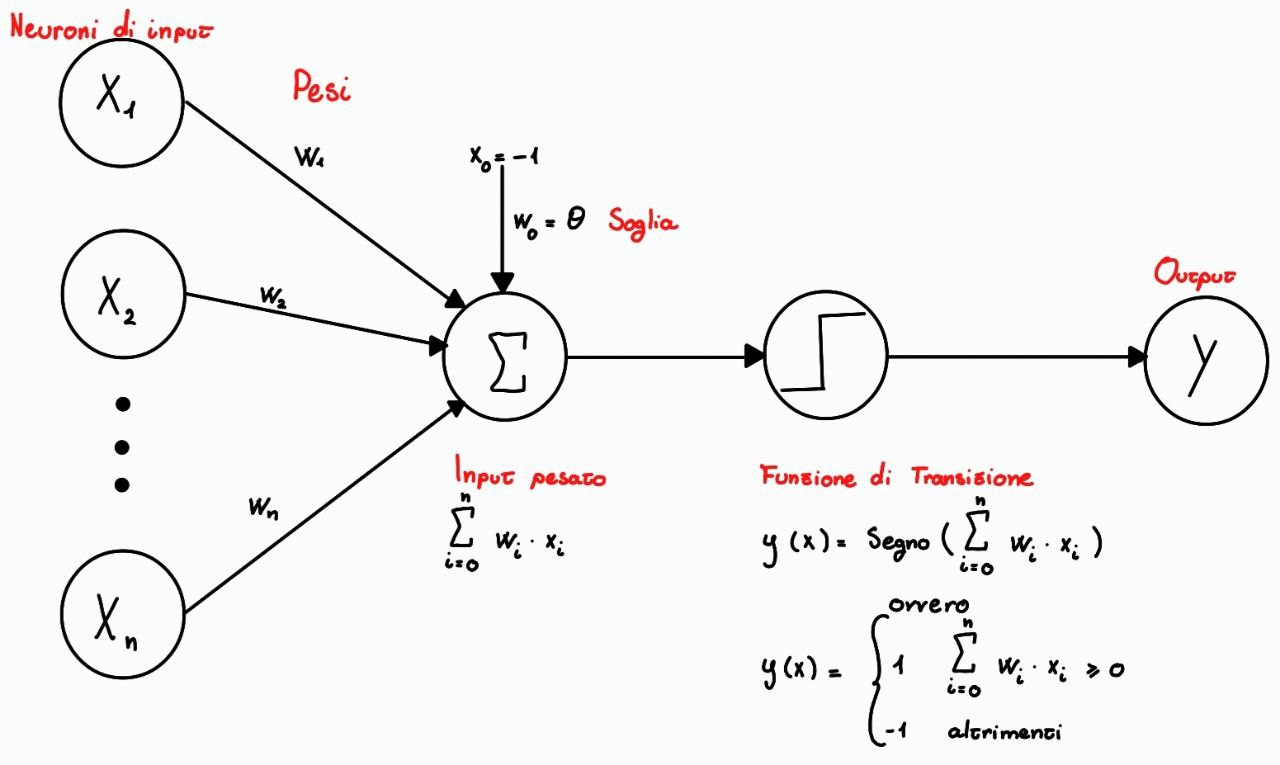
\includegraphics[width=0.7\textwidth]{img/reti/percettrone.png}
    \caption{Rappresentazione grafica del percettrone}
\end{figure}

Un percettrone è composto da un vettore di input $x_i$, ognuno con associato un
peso $w_i$. Oltre a questi, esso prende in input una soglia $\theta$, la quale è
trattata come il peso di una unità di input in stato fisso $x_0 = -1$. La transizione
di stato è determinata dal risultato del prodotto interno tra il vettore dei
pesi $\textbf{w}$ e il vettore degli stati di input $\textbf{x}$. Da un punto di
vista geometrico, il vettore dei pesi determina un iperpiano che separa i possibili
vettori di input in due classi, a seconda che formino con $\textbf{w}$ un angolo
acuto oppure ottuso.

Solitamente coi percettroni si parla di learning supervisionato.

Il processo di apprendimento di un percettrone parte assegnando in modo casuale
i pesi agli input. Questi pesi verranno modificati nella fase di apprendimento.

Se assumiamo che l'obiettivo è quello di separare i vettori in input in due classi
$A$ e $B$, possiamo utilizzare la seguente procedura per raggiungere questo scopo.
Si sottomette una sequenza infinita $\{x_k\}$ di vettori tale che ve ne siano un
numero infinito sia di $A$ che di $B$. Per ogni $x_k$ la rete calcola la risposta
$y_k$. Se la risposta è errata, si modificano i pesi nel seguente modo:
\begin{itemize}
    \item Incremento i pesi delle unità di input attive se si è risposto 0 anziché 1.
    \item Decremento i pesi delle unità di input attive se si è risposto 1 anziché 0.
\end{itemize}
\begin{equation}
    w' = w \pm x
\end{equation}

Vediamo due teoremi utili per lo studio dell'apprendimento del percettrone su due
classi $A$ e $B$, banalmente rappresentanti, nella nostra situazione binaria e
semplificata, il caso in cui si abbia il neurone che emette il segnale o altrimenti.
Nel nostro caso le classi sono discriminabili.
\begin{teorema}[\textbf{Teorema della convergenza}]
    Comunque si scelgano i pesi iniziali, se le classi $A$ e $B$ sono discriminabili,
    la procedura di apprendimento termina dopo un numero finito di passi.
\end{teorema}
\begin{teorema}[\textbf{Teorema di Minsky e Papert}]
    La classe delle forme discriminabili da un percettrone semplice è limitata
    alle forme linearmente separabili.
\end{teorema}

\begin{teorema}
    Se l'insieme degli input estesi è partito in due classi linearmente separabili
    $A$ e $B$ allora è possibile trovare un vettore di pesi $w$ tale che:
    \begin{equation}
        \begin{array}{ccc}
            \textbf{w} \cdot \textbf{x} \geq 0 & se & x \in A \\
            \textbf{w} \cdot \textbf{x} < 0    & se & x \in B
        \end{array}
    \end{equation}
\end{teorema}

Vediamo ora una nuova regola per aggiornare i pesi del percettrone:
\begin{equation}
    w'_i = w_i + \Delta w_i = w_i + \eta \cdot (t - y) \cdot x_i
\end{equation}
dove: \begin{itemize}
    \item $t$ rappresenta il valore del target.
    \item $y$ rappresenta l'output del percettrone.
    \item $\eta$ rappresenta il learning rate.
\end{itemize}

Così facendo si aggiornano i pesi del percettrone quando esso sbaglia la risposta.
Usando questa regola, l'algoritmo converge alla classificazione corretta se i
dati del training sono linearmente separabili e se $\eta$ assume un valore abbastanza piccolo.
\subsection{Discesa del gradiente}
Si consideri ora una unità lineare, con stati continui e un output calcolato come:
\begin{equation}
    y = w_0 + w_1x_1 + \dots + w_nx_x
\end{equation}
Una possibile strategia di apprendimento per questo modello consiste nel minimizzare
una opportuna funzione dei pesi $w_i$. Questo risultato può essere ottenuto cercando
di minimizzare l'errore ottenuto sul training set usando la discesa del gradiente:
\begin{equation}
    w' = w - \eta \cdot \nabla E[\textbf{w}]
\end{equation}
dove posso approssimare la discesa del gradiente come:
\begin{equation}
    \sum_d (t_d - y_d) (- x_i)
\end{equation}
Per effettuare questo aggiornamento abbiamo due modalità:
\begin{itemize}
    \item \textbf{Modalità Batch}: dove l'aggiornamento dei pesi viene calcolato
          rispetto all'intero insieme $D$.
          \begin{equation}
              w = w - \eta \cdot \nabla E_D[w] \ \text{con} \ E_D[w] = \frac{1}{2} \sum_{d \in D} (t_d - y_d)^2
          \end{equation}
          Esiste una variante chiamata \textbf{mini batch} che consiste nel dividere
          il dataset in $n$ porzioni e aggiornare i pesi ogni volta che si è
          analizzato un batch.
    \item \textbf{Modalità incrementale}: dove l'aggiornamento dei pesi viene
          calcolato rispetto a singoli esempi $d$.
          \begin{equation}
              w = w - \eta \cdot \nabla E_d[w] \ \text{con} \ E_d[w] = \frac{1}{2} (t_d - y_d)^2
          \end{equation}
          Questa modalità può approssimare la discesa del gradiente con la
          modalità Batch arbitrariamente se $\eta$ è abbastanza piccolo.
\end{itemize}

Rispetto a quanto visto per il percettrone la discesa lungo il gradiente converge
all'ipotesi con il minimo errore quadratico se $\eta$ è abbastanza basso, anche
per dati di training molto rumorosi.
\section{Reti neurali}
Fino ad ora abbia studiato il comportamento del singolo neurone, ma come per il
cervello umano, la forza di questo approccio è data dall'unione di più neuroni.
Per realizzare questo risultato la soluzione consiste nel collegare i neuroni in
modo da ottenere una struttura a grafo aciclico orientato. Così facendo, l'output
di un neurone diventa l'input di un altro.

Le reti neurali così composte hanno delle caratteristiche strutturali come:
\begin{itemize}
    \item hanno un gran numero di unità.
    \item permettono operazioni elementari.
    \item hanno un alto livello di interconnessione.
\end{itemize}
e delle caratteristiche dinamiche:
\begin{itemize}
    \item Si hanno cambiamenti di stato in funzione dello stato dei neuroni collegati
          in input.
    \item Si ha una funzione di uscita per ogni unità.
    \item Si ha la modifica dello schema di connessione, tramite la modifica dei
          pesi, per l'apprendimento.
\end{itemize}

L'output di un neurone è uno stato per un altro neurone. Si hanno alcuni elementi
caratterizzanti di una rete neurale:
\begin{itemize}
    \item Il tipo di unità.
    \item La topologia, ovvero la direzione delle connessioni, il numero di neuroni, $\dots$
    \item Le modalità di attivazione.
    \item Un algoritmo di apprendimento con lo studio dei pesi.
\end{itemize}

L'apprendimento di un neurone modifica i pesi sinaptici. Se due neuroni connessi
sono per più volte di seguito contemporaneamente attivi, il peso della sinapsi aumenta.
\begin{figure}[!ht]
    \centering
    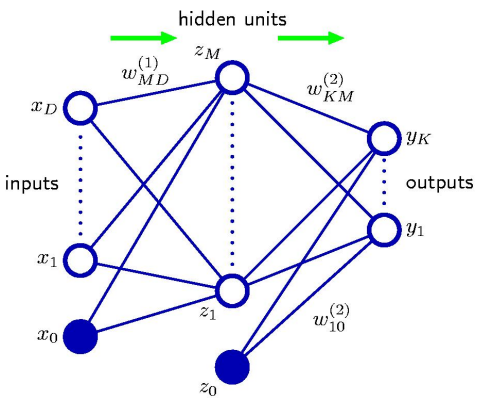
\includegraphics[width=0.6\textwidth]{img/reti/rete.png}
    \caption{Rete Neurale multi strato}
\end{figure}

Dal punto di vista formale, dovendo espandere le definizioni fatte nel caso del
singolo neurone a più neuroni, si lavora con:
\begin{itemize}
    \item $D$ le variabili di input $x_1, \dots, x_D$.
    \item Una matrice dei pesi $W$, con i valori indicati tramite $w_{ij}$, per
          gli archi che collegano i neuroni. I pesi sono i pesi correnti.
    \item Un vettore delle soglie $\Theta$, con i valori indicati tramite $\theta_i$,
          una per ogni neurone.
    \item L'input netto per il neurone $i$ al tempo $t$, indicato con:
          \begin{equation}
              n_i(t) = \sum_{j = 1}^n w_{ij} \cdot x_j(t) - \theta_i
          \end{equation}
          quindi si ha che la soglia influisce già nell'input del neurone e quindi
          $\theta_i$ viene considerata come soglia di azzeramento del valore entrante.
    \item La funzione di transizione indicata con:
          \begin{equation}
              s_i(t + 1) = g(n_i(t))
          \end{equation}
    \item $M$ ovvero il numero delle unità di attivazione nascoste:
          \begin{equation}
              a_j = \sum_{i = 1}^D w_{ji}^{(1)}x_i + w_{j0}^{(1)}
          \end{equation}
          dove $j = 1, \dots, M$.
    \item $z_j = h(a_j)$ come le funzioni di attivazione nascoste.
    \item $K$ ovvero il numero delle unità di attivazione in output:
          \begin{equation}
              a_k = \sum_{i = 1}^M w_{ki}^{(2)}x_i + w_{k0}^{(2)}
          \end{equation}
          dove $k = 1, \dots, K$.
    \item Indichiamo con $y_k = \sigma(a_k)$ la funzione di attivazione dell'ultimo strato.
          \begin{equation}
              y_k(\textbf{x}, \textbf{w}) = \sigma \left(\sum_{j = 1}^M w_{kj}^{(2)} \cdot h \left(\sum_{i = 1}^D w_{ji}^{(1)}x_i + w_{j0}^{(1)}\right) + w_{k0}^{(2)}\right)
          \end{equation}
\end{itemize}

I singoli \textit{percettroni} ci permettono di costruire delle frontiere di
separazione lineari, questo però limita l'applicabilità di questa tecnica. Nel
caso in cui si ha la volontà di costruire frontiere di separazione non lineari è
necessario combinare più neuroni $u_i$, anche posizionati in strati intermedi tra
input e output, andando a formare una rete.

Per questa modifica si passa dalla funzione di attivazione a gradino a una funzione
di attivazione derivabile, ovvero la sigmoide:
\begin{equation}
    \sigma(x) = \frac{1}{1 + e^{-x}}
\end{equation}
Questa scelta viene fatta per semplificare la fase di aggiornamento dei pesi.

A questo punto, per ogni configurazione in ingresso al primo strato $x$, la rete
calcola una configurazione $y$ dell'ultimo strato.

L'obiettivo è fissata una mappa $f$ tra configurazioni di ingresso e di uscita,
sulla base di una sequenza di stimoli $x_k$, la rete cambia i pesi $w_{ij}$ in
modo che, dopo un numero finito $s$ di passi l'uscita $y_k$ coincida con $f(x_k)$
per ogni $k > s$, almeno approssimativamente. Il criterio di apprendimento della
rete consiste nel minimizzare la discrepanza tra il target atteso e la previsione della rete.

Nella fase di addestramento l'obiettivo è quello di determinare i pesi $w$ da
assegnare alle connessioni della rete partendo da un training set. La procedura di
apprendimento è composta da due step:
\begin{enumerate}
    \item Valutare il gradiente dell'errore $\nabla E(w)$ rispetto ai pesi $w_1, \dots, w_T$.
    \item Usare il vettore di derivate ottenuto per calcolare i nuovi pesi.
\end{enumerate}
\begin{equation}
    w^{(\tau + 1)} = w^{(\tau)} - \eta \cdot \nabla E(w^{(\tau)})
\end{equation}

Usando un \textbf{Computational Graph} possiamo rappresentare una funzione composta
come un grafo aciclico orientato dove ogni nodo rappresenta una funzione o un
operazione e ogni arco rappresenta l'input per il nodo.

Possiamo calcolare la derivata di una funzione composta $f(g(h(x)))$ come:
\begin{equation}
    \frac{df}{dx} = \frac{df}{dg} \cdot \frac{dg}{dh} \cdot \frac{dh}{dx}
\end{equation}
\subsection{Backpropagation}
Quando si lavora con le reti l'aggiornamento dei pesi risulta più complicato
rispetto a quando si lavora con il singolo neurone. Infatti, nel caso delle reti
l'errore lo sappiamo solamente alla fine. Risulta quindi difficile il processo di
aggiornare gli stati intermedi.

Quando si lavora con più strati, l'aggiornamento dei pesi viene ottenuto per mezzo
di una derivata della funzione composta.

Abbiamo quindi l'algoritmo di \textbf{Backpropagation} che si divide in 5 passi:
\begin{enumerate}
    \item \textbf{Input}: al neurone di input $u_j$ viene assegnato lo stato $x_j$.
    \item \textbf{Propagazione}: si calcola lo stato dei neuroni nascosti o di output $u_j$:
          \begin{equation}
              s_j = f_j(n_j)
          \end{equation}
          dove $n_j$ è l'input netto al neurone $u_j$ e si calcola come:
          \begin{equation}
              n_j = \sum_{i = 0}^n w_{ij} \cdot s_i
          \end{equation}
    \item \textbf{Confronto}: per ogni neurone di output $u_j$, noto l'output
          atteso $t_j$, si calcola:
          \begin{equation}
              \delta_j = f'_j(n_j) \cdot (t_j - y_j)
          \end{equation}
          Possiamo vedere la propagazione in avanti nella rete si ottiene come
          moltiplicazione tra matrici. In particolare, ogni strato è in funzione
          dello strato precedente.
    \item \textbf{Retropropagazione dell'errore}: per ogni neurone nascosto $u_j$,
          si calcola:
          \begin{equation}
              \delta_j = f_j'(n_j) \cdot \left( \sum_{h} w_{jh} \cdot \delta_h \right)
          \end{equation}
    \item \textbf{Aggiornamento dei pesi}: si ha:
          \begin{equation}
              w_{ij} = w_{ij} + \eta \cdot \delta_i \cdot s_j
          \end{equation}
\end{enumerate}

Vediamo quindi una possibile implementazione dell'algoritmo:
\begin{algorithm}[H]
    \begin{algorithmic}
        \Function{Backpropagation}{}
        \State \textit{inizializzo ogni $\Delta w_i$ ad un valore piccolo casuale}
        \While {\textit{non raggiungimento della condizione di terminazione}}
        \For {\textit{ogni esempio $\langle (x_1,\ldots, x_n),t\rangle$}}
        \State \textit{immetto l'input $( x_1, \ldots x_n)$ nella rete e calcolo
            $y_k$}
        \For {\textit{ogni unità di output $k$}}
        \[\delta_k=y_k\cdot(1-y_k)\cdot(t_k-y_k)\]
        \EndFor
        \For {\textit{ogni unità nascosta $h$}}
        \[\delta_h=y_h\cdot(1-y_h)\cdot\sum_k w_{hk}\delta_k\]
        \EndFor
        \For {\textit{ogni peso $w_{ij}$}}
        \[w_{ij}=w_{ij}+\Delta w_{ij},\mbox{ con } \Delta w_{ij}=\eta\cdot\delta_j\cdot x_{ij}\]
        \EndFor
        \EndFor
        \EndWhile
        \State \textit{aggiorno i pesi:}
        \[w_i=w_i+\Delta w_i\]
        \EndFunction
    \end{algorithmic}
    \caption{Algoritmo di Backpropagation}
\end{algorithm}

Si trova però un minimo locale e non globale e spesso include termini di \textit{momento}
per cambiare la formula dell'aggiornamento dei pesi del tipo:
\begin{equation}
    \delta w_{ij}(n) = \eta \cdot \delta_j \cdot x_{ij} + \alpha \cdot \Delta w_{ij} (n - 1)
\end{equation}
in modo da avere una sorta di inerzia per la variazione dei pesi. Esistono
tecniche che permettono di "uscire" dai minimi locali.

Si minimizzano gli errori sugli esempi di training ma si rischia l'overfitting.

Tutti questi fattori comportano un addestramento lento, ma dopo l'addestramento
si ha una rete veloce.
\subsection{Overfitting}
Più la rete è ricca di neuroni e pesi e più può imparare semplicemente "fotografando"
nella sua memoria le istanze, questo porta a una situazione di overfitting.

Un idea per limitarlo consiste nel penalizzare la rete durante il training, ovvero
costringo la rete a generalizzare cogliendo regolarità nelle istanze, invece di
"fotografarle". In generale queste sono dette tecniche di \textbf{regolarizzione}.

Esistono diverse tecniche per limitare l'overfitting, una di queste è chiamata
\textbf{dropout}. Questa tecnica consiste nello spegnere un determinato numero di
neuroni in modo da obbligare la rete a generalizzare.
\subsection{Utilizzi}
Uno degli utilizzi delle reti neurali è quello di ridurre la dimensionalità dei
dati mantenendo le informazioni essenziali. Questo risultato può essere ottenuto
anche con tecniche che non richiedono l'uso di reti neurali, ad esempio utilizzando
una tecnica nota come \textbf{PCA} (\textit{Principal Component Analysis}). L'idea
dietro questa tecnica consiste nel trovare una trasformazione lineare delle
caratteristiche che massimizza la varianza o minimizza l'errore quadratico di
ricostruzione.

Gli \textbf{Autoencoder} sono delle reti neurali che mi permettono di codificare
gli input utilizzando poche informazioni. Questo particolare modello di rete neurale
è unsupervised e viene addestrata in modo che l'input sia uguale all'output. Per
riuscire a ridurre la codifica dell'input la rete è composta da due parti che sono
collegate tra di loro una dopo l'altra:
\begin{itemize}
    \item \textbf{Encoder}: si occupa di prendere l'input e ridurlo di dimensionalità.
    \item \textbf{Decoder}: partendo dalla codifica in pochi bit ricostruisce l'input originale.
\end{itemize}
\begin{figure}[!ht]
    \centering
    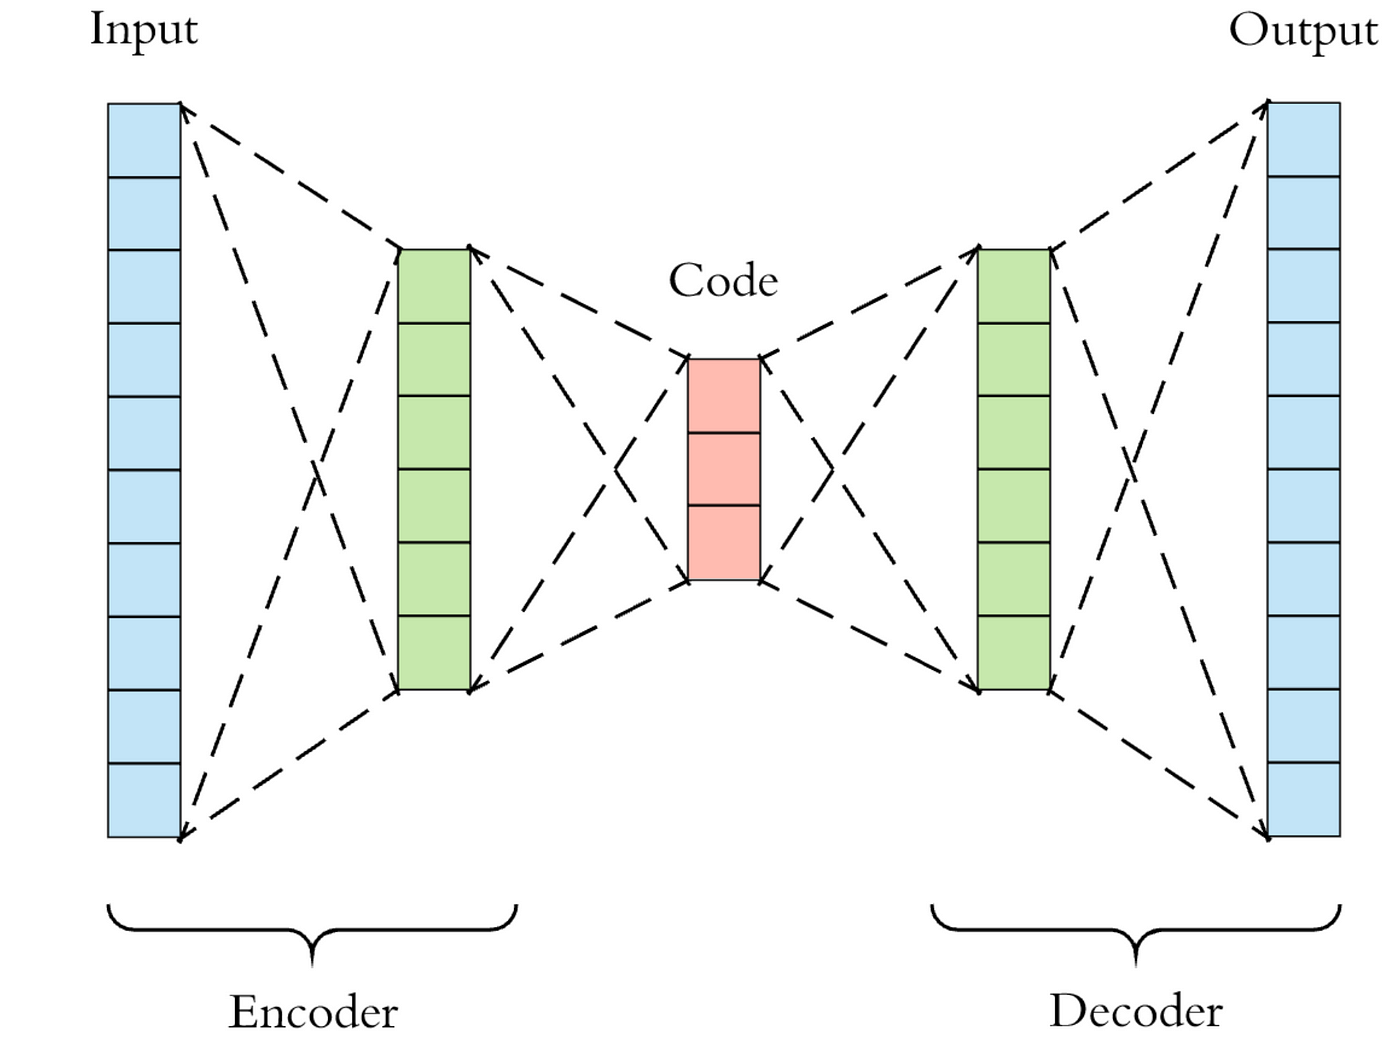
\includegraphics[width = 0.6\textwidth]{img/reti/autoencoder.png}
    \caption{Struttura di un Autoencoder}
\end{figure}

Oltre a questo si cerca di trasformare features categoriche in features numeriche
in modo da semplificare i processi di apprendimento.
\subsection{Limiti}
Si hanno quindi i seguenti limiti:
\begin{itemize}
    \item Mancanza di teoremi generali di convergenza.
    \item Può portare in minimi locali di E.
    \item Difficoltà per la scelta dei parametri.
    \item Scarsa capacità di generalizzazione.
\end{itemize}
Si possono però avere varianti che permettono di migliorare il modello tramite:
\begin{itemize}
    \item Un tasso di apprendimento adattivo: $\eta = g(\nabla E)$
    \item Range degli stati da $-1$ a $1$.
    \item L'uso di termini di momento.
    \item Deviazioni dalla discesa più ripida.
    \item Variazioni nell'architettura (numero di strati nascosti)
    \item Inserimento di connessioni all'indietro.
\end{itemize}

\begin{osservazione}
    Rispetto alberi decisionali si ha:
    \begin{itemize}
        \item Le reti neurali sono più lente in fase di apprendimento ma uguali
              in fase di esecuzione.
        \item Le reti neurali hanno una migliore tolleranza del rumore.
        \item Le reti neurali risultano più complesse da capire.
    \end{itemize}

    Si nota che ne le reti neurali ne gli alberi decisionali possono usare della
    conoscenza a priori.
\end{osservazione}